\section{Zielsetzung}
\label{sec:Zielsetzung}

In diesem Versuch sollen die Grundlagen der Lasertechnik kennengelernt
werden. Hierzu werden einige Eigenschaften des HeNe-Lasers experimentell
überprüft.

\section{Theorie}
\label{sec:Theorie}
% Vorschlag für den Beginn, damit nicht andauernd zitiert werden muss.
Die folgende theoretische Beschreibung von optischen Geräten wie Laser ist aus den Quellen
\cite{anleitung} und \cite{eichler} entnommen,
sofern nicht anders gekennzeichnet.

Laser erzeugen einen
Lichtstrahl mit hoher Kohärenz, Intensität und Polarisation. Für eine theoretischen
Beschreibung der Funktionsweise werden Wechselwirkungen eines Strahlenfeldes mit einem
System aus Atomen zu analysieren. Ein theoretisches Modell hierfür bietet ein
Zweiniveausystem.

\subsection{Zweiniveausystem}
Ein einfaches Modell zur Beschreibung eines Systems aus Atomen ist das Zweiniveausystem,
welches aus zwei Zuständen $\left| 1 \right>$ und $\left| 2 \right>$ mit entsprechenden
Eigenwerten $E_1$ und $E_2$ ($E_1<E_2$) besteht.
Durch Absorption und Emission eines Photons mit
Energie $h\nu=E_2-E_1$ kann ein Elektron zwischen den Zuständen wechseln.
Dabei sind folgende Prozesse für die Lasertechnik wichtig:
\begin{itemize}
  \item induzierte Absorption:
  Hier wird durch Absorption eines Photons das System in Zustand $\left| 2 \right>$
  gehoben. Die Wahrscheinlichkeit, mit der dieser Prozess stattfindet, wird beschrieben
  durch
  \begin{equation}
    P_{1\rightarrow 2} = B_{1\rightarrow 2}\cdot \rho(\nu).
  \end{equation}
  Dabei stellt $P_{1\rightarrow 2}$ die Übergangswahrscheinlichkeit, $B_{1\rightarrow 2}$ den
  Einsteinkoeffizienten für die induzierte Absorption und $\rho(\nu)$ die spektrale Energiedichte
  eines externen Strahlungsfeldes da.
  \item induzierte Emission:
  Hierbei stimmt das induzierte Photon in Energie, Phase und Ausbreitungsrichtung
  mit einem anregenden Photon überein. Es kann eine analoge Beschreibung wie bei der
  induzierten Absorption verwendet werden.
  Somit wird die Übergangswahrscheinlichkeit durch
  \begin{equation}
    P_{2\rightarrow 1} = B_{2\rightarrow 1}\cdot\rho(\nu)
  \end{equation}
  definiert. $B_{2\rightarrow 1}$ stellt hier den Einsteinkoeffizienten der induzierten
  Emission da.
  \item spontane Emission:
  Auch in Abwesenheit eines externen Strahlenfeldes kann ein Photon emittiert werden.
  Dabei gilt die Beziehung
  \begin{equation}
    P_s = A_{2\rightarrow 1}
  \end{equation}
  mit dem Einsteinkoeffizienten $A_{2\rightarrow 1}$.
\end{itemize}

Befindet sich ein System im thermischen Gleichgewicht, so kann es durch die
Besetzungszahlen $n_i$ der Niveaus beschrieben werden. Diese folgen der
Boltzmann-Statistik
\begin{equation}
    n_i = \frac{g_in}{Z}\exp\left(-\frac{E_i}{k_\text{B}T}\right).
\end{equation}
Als $n$ wird die Gesamtzahl der Systeme, $g_i$ das statistische Gewicht dess Zustandes
$\left| i \right>$ und Zals die Zustandssumme bezeichnet. Durch den Einsatz
eines Lasers soll dafür gesorgt werden, das eine dauerhafte Verstärkung des
Strahlungsfeldes entsteht.

\subsection{Aufbau und Funktionsweise eines Lasers}
Das Wort Laser steht für \enquote{Light Amplification by Stimulated Emission of
Radiation}. Ein Laser besteht prinzipiell aus drei Teilen:
Dem aktiven Lasermedium, einer Pumpquelle und einem Resonator.
% Dieser schematische ist in Abbildung \ref{pic:laser} zu sehen.
Abbildung \ref{pic:laser} zeigt eine schematische Darstellung eines Lasers.
\begin{figure}[htb]
  \centering
  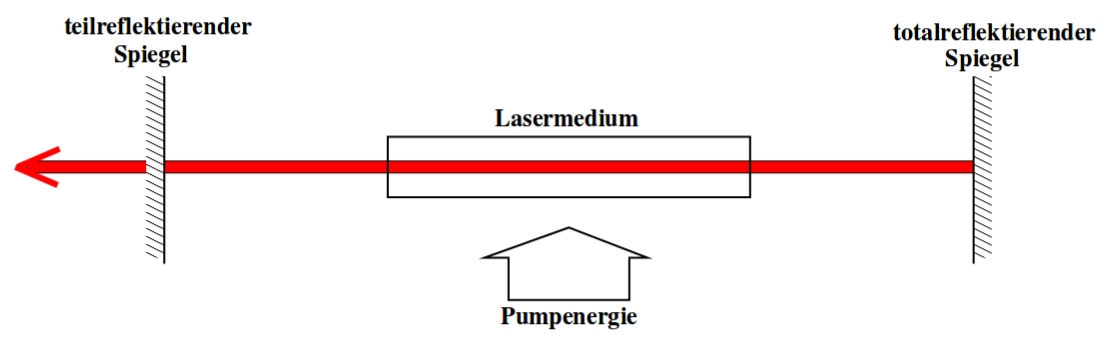
\includegraphics[width=0.8\textwidth]{content/prinzip_laser.png}
  \caption{Schematischer Aufbau eines Lasers mit Pumpquelle, aktivem Medium und Resonator \cite{anleitung}.}
  \label{pic:laser}
\end{figure}
Eine Pumpquelle stellt eine sogenannte Besetzungsinversion her.
Diese bedeutet, dass mehr Elektronen in einem angeregten Zustand sind, als
im Grundzustand. Ohne Pumpquelle wäre dies nicht möglich, da wie oben
dargestellt das statistische Gewicht des Grundzustands größer ist.
% Um mindestens einen angeregten Zustand mehr im aktiven zu haben wie Grundzustände,
% wird eine Pumpquelle verwendet um diese Besetzungsinverssion herzustellen.
Daraufhin tritt in dem Lasermedium oder auch aktiven Medium häufiger
induzierte als spontane Emission auf und das
Strahlungsfeld wird verstärkt.
Um diese Verstärkung zu maximieren, befindet sich das Lasermedium zwischen
zwei gegenüber liegenden Spiegeln, welche das Licht reflektieren und somit
den Laufweg der Photonen im Lasermedium maximieren.
% Damit der Laufweg der Photonen möglichst groß wird, verlängert
% der Resonator genau diesen durch zwei gegenüberliegende Spiegel.
Einer dieser Spiegel ist halbdurchlässig,
um einen erzeugten Strahl auskoppeln zu können. Der andere ist vollständig reflektierend.
Dabei werden durch eine konfokale Anordnung Verluste minimiert,
die durch eine Abweichung des Strahlenganges vom optimalen Weg entstehen.
% Ein langer Laufweg ist wichtig, da so ein Photon öfters durch das Lasermedium gelangen kann
% und dadurch weitere Emissionen bewirkt.
Im Resonator können nur Wellenlängen verstärkt werden, welche die Bedingung
\begin{equation}
  \lambda = \frac{2L}{n} \text{ mit } n\in\mathds{N}
\end{equation}
erfüllen.
Hierbei ist $L$ der Abstand zwischen den Spiegeln und n der Index der Moden.
Diese Bedingung begründet sich aus der Bedingung an stehende Wellen,
welche die Elektronenfunktionen zwischen den Resonatorspiegeln ausbilden.
Durch diese Bedingung tritt eine Selektion der Wellelängen auf, die betrachtet werden können.
Innerhalb eines durch den optischen Dopplereffekt auftretenden natürlichen Spektrums
sind dies die longitudinale Moden.

Treten stationäre Intenstiätsverteilungen durch Beugungseffekte an Unebenheiten
der Spiegel senkrecht zur Rotationachse auf, so werden diese als transversale oder
TEM-Moden (\textit{transversal electromagnetic}) bezeichnet.

Wird die Intensität $I_{00}$ der Grund- oder Fundamentalmode $T_{00}$ betrachtet,
so folgt sie einer Gaußverteilung der Form
\begin{equation}
  I_{00} = I_0 \exp\left(-2\left(\frac{d-d_0}{w}\right)^2\right).
  \label{eqn:t00}
\end{equation}
$w$ wird als Radius der Fundamentalmode und $d$ als senkrechter Abstand zur Resonatorachse
bezeichnet.
Die nächsthöhere $T_{01}$ Mode wird beschrieben durch
\begin{equation}
  I_{01}(d) = I_{0,1}\text{e}^{-2\left(\frac{d-d_{0,1}}{w_1}\right)^2}+I_{0,2}\text{e}^{-2\left(\frac{d-d_{0,2}}{w}\right)^2}.
\label{eqn:t10}
\end{equation}
Es tritt hier eine theoretisch nicht erwartete Asymmetrie in der Höhe der beiden Maxima,
d.h. $I_{0,1} \neq I_{0,2}$ auf.

Stabile Moden treten auf, wenn die Stabilitätsbedingung
\begin{equation}
  0\leq g_1g_2\leq 1
\end{equation}
auftritt. Dabei beschreibt
\begin{equation}
  g_i = 1 - \frac{L}{r_i}
\end{equation}
mit dem Krümmungsradius des $i$-ten Spiegels $r_i$.
In Abbildung \ref{fig:stabilität} ist das Produkt $g_1g_2$
als Funktion des Spiegelastandes $L$  für $r_2 = \SI{1400}{\metre}$ dargestellt.
Wird ein ebener Spiegel ("$r_1 = \infty$") betrachtet, so ergibt sich eine
 Bedingung für $L$ von
\begin{equation}
  \SI{0}{\metre} \leq L \leq \SI{1.4}{\metre}.
\end{equation}
Ein Spiegel mit $r_1 = \SI{1400}{\milli\metre}$ ergibt
\begin{equation}
    \SI{0}{\metre} \leq L \leq \SI{2.8}{\metre}.
\end{equation}

\begin{figure}
  \centering
  \includegraphics[width=0.6\textwidth]{build/stabilitaet.pdf}
  \caption{Darstellung der Stabilitätsparameter in Abhängigkeit der
  Resonatorlänge $L$.}
  \label{fig:stabilität}
\end{figure}
\FloatBarrier

\subsection{Helium-Neon-Laser}
\label{sec:Helium-Neon-Laser}
Bei einem Helium-Neon-Laser (HeNe-Laser)
besteht das Resonatormedium aus fünf Teilen Neon und einem Teil Helium, welches
bei einem Druck von $\SI{1}{\milli\bar}$ in einem Glaskolben eingeschlossen ist.
Durch Gasentladung wird ein Heliumkern in die $2^1s$ und $2^3s$ Zustände angeregt,
welches durch Stöße zweiter Art die $5s$ und $4s$ Zustände der Neonatome anregt.
Dies ist in Abbildung \ref{fig:HeNe} dargestellt.
\begin{figure}
  \centering
  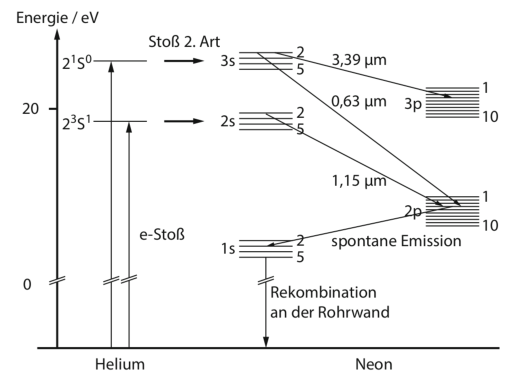
\includegraphics[width=0.6\textwidth]{content/HeNe.pdf}
  \caption{Schematische Darstellung der Übergänge zur stimulierten
  Emission eines HeNe-Lasers \cite[68]{eichler}.}
  \label{fig:HeNe}
\end{figure}

Da der $5s$ Zustand des Heliums eine größere mittlere Lebensdauer hat als der
$3s$ Zustand, ist die Besetzungsinversion erfüllt und wahrscheinlicher als
spontane Emissionen. Die bei diesem Übergang auftretende Spektrallinie zwischen
den beiden Neonatomen liegt bei $\lambda = \SI{632.8}{\nano\metre}$ und damit
im sichtbaren roten Bereich des elektromagnetischen Spektrums.
